% =====================================================================
%  Capítulo 4. Problemas del MCO con datos financieros
% =====================================================================
\chapter[Problemas del MCO con datos financieros]{Problemas del MCO con datos financieros: heterocedasticidad, autocorrelación y cambios estructurales}\label{cap:robustos}

\section*{Objetivos de aprendizaje}
Al terminar este capítulo, el lector podrá:
\begin{enumerate}[label=\arabic*.,leftmargin=*]
  \item Explicar por qué la heterocedasticidad y la autocorrelación no sesgan los estimadores MCO pero
        invalidan sus errores estándar clásicos, y cuantificar el error.
  \item Derivar y calcular los errores estándar robustos de White (HC0, HC1) y de Newey-West (HAC).
  \item Aplicar las pruebas de Breusch-Pagan y de White, y una prueba de autocorrelación robusta a la
        heterocedasticidad.
  \item Reconocer el problema de las regresiones con horizontes traslapados y corregir su inferencia.
  \item Contrastar cambios estructurales con fecha conocida (Chow), con fecha desconocida (sup-F) y de
        forma secuencial (CUSUM).
\end{enumerate}

\section*{Motivación}
Los Capítulos~\ref{cap:hechos} y~\ref{cap:capm} dejaron dos cuentas pendientes. En el primero, la prueba de
Ljung-Box rechazó que los rendimientos del Brent no estuvieran autocorrelacionados ($p=0{,}004$), y
advertimos que la prueba podía estar engañada por la volatilidad cambiante. En el segundo, calculamos
estadísticos $t$ para las alfas y betas del CAPM con fórmulas que suponen varianza constante y errores no
correlacionados, dos supuestos que los datos financieros violan sistemáticamente.

El problema es general. MCO sigue siendo un buen estimador con datos financieros, pero sus errores estándar
clásicos pueden estar muy equivocados, y con ellos todas las pruebas de hipótesis y los intervalos de
confianza. Este capítulo muestra cuánto se equivocan, cómo corregirlos y qué ocurre con las conclusiones de
los capítulos anteriores cuando se corrigen. Cierra con otro problema típico de las series financieras
largas: que los parámetros cambien en el tiempo.

\paragraph{Datos del capítulo.} Reutilizamos la base de Kenneth French (1949--2017), el Brent diario
(1987--2026) y el S\&P 500 mensual de Shiller con dividendos (1871--2023). Las simulaciones de Monte Carlo
de la teoría están en \texttt{codigo/Python/cap04\_figuras\_teoria.py}, con semilla fija.

% ---------------------------------------------------------------------
\section{Heterocedasticidad}
% ---------------------------------------------------------------------

\begin{definicion}[Heterocedasticidad]
En el modelo $y_t=\alpha+\beta x_t+\varepsilon_t$ con $\E[\varepsilon_t\mid x]=0$, hay
\emph{heterocedasticidad} si la varianza condicional $\sigma^2_t=\Var(\varepsilon_t\mid x)$ cambia entre
observaciones.
\end{definicion}

En el modelo de mercado hay una razón económica para esperarla: en los meses de grandes movimientos del
mercado (crisis, pánicos, burbujas) también son grandes los movimientos idiosincráticos de cada industria.
La varianza del residuo crece entonces con $|x_t|$, y la nube de puntos tiene forma de embudo
(Figura~\ref{fig:hetero}, izquierda).

\begin{proposicion}[MCO con heterocedasticidad]\label{prop:mcohetero}
Si los errores no están correlacionados pero $\Var(\varepsilon_t\mid x)=\sigma_t^2$, entonces $\hat\beta$
sigue siendo insesgado, pero
\[
  \Var(\hat\beta\mid x)=\frac{\sum_t(x_t-\bar x)^2\sigma_t^2}{S_{xx}^2},
\]
que en general es distinta de la fórmula clásica $\sigma^2/S_{xx}$. En muestras grandes, el cociente entre
la varianza verdadera y la que estima la fórmula clásica tiende a
\[
  \frac{\E\bigl[(x_t-\mu_x)^2\sigma_t^2\bigr]}{\Var(x_t)\,\E[\sigma_t^2]},
\]
que es mayor que 1 cuando la varianza del error es mayor en las observaciones con $x_t$ alejado de su media.
\end{proposicion}

\begin{proof}
La demostración del Teorema~\ref{teo:varmco} mostró, sin usar ningún supuesto sobre la varianza, que
\begin{align*}
  \hat\beta &= \beta+\sum_tc_t\varepsilon_t, \qquad c_t=\frac{x_t-\bar x}{S_{xx}},
\end{align*}
de modo que $\E[\hat\beta\mid x]=\beta$: el insesgamiento se mantiene. Como los errores no están
correlacionados:
\begin{align*}
  \Var(\hat\beta\mid x) &= \sum_tc_t^2\,\sigma_t^2\\
                        &= \frac{\sum_t(x_t-\bar x)^2\,\sigma_t^2}{S_{xx}^2} .
\end{align*}
La fórmula clásica estima $s^2/S_{xx}$, y $s^2$ converge al promedio de las varianzas, $\E[\sigma_t^2]$. El
cociente entre ambas, dividiendo numerador y denominador entre $T$, es
\begin{align*}
  \frac{\Var(\hat\beta\mid x)}{s^2/S_{xx}}
    &= \frac{\sum_t(x_t-\bar x)^2\,\sigma_t^2}{S_{xx}^2}\cdot\frac{S_{xx}}{s^2}\\
    &= \frac{\frac1T\sum_t(x_t-\bar x)^2\,\sigma_t^2}{\frac1TS_{xx}\cdot s^2}\\
    &\longrightarrow \frac{\E\bigl[(x_t-\mu_x)^2\sigma_t^2\bigr]}{\Var(x_t)\,\E[\sigma_t^2]} .
\end{align*}
Por último, el numerador se descompone así:
\begin{align*}
  \E\bigl[(x_t-\mu_x)^2\sigma_t^2\bigr] &= \E\bigl[(x_t-\mu_x)^2\bigr]\,\E[\sigma_t^2]+\Cov\bigl((x_t-\mu_x)^2,\sigma_t^2\bigr)\\
                                        &= \Var(x_t)\,\E[\sigma_t^2]+\Cov\bigl((x_t-\mu_x)^2,\sigma_t^2\bigr),
\end{align*}
y el cociente es mayor que 1 si y solo si esa covarianza es positiva.
\end{proof}

\subsection{El estimador de White}

En notación matricial, con $\bm X$ la matriz $T\times k$ de regresores (incluida la columna de unos),
$\hat{\bm\beta}=(\bm X'\bm X)^{-1}\bm X'\bm y$ y $\hat{\bm\beta}-\bm\beta=(\bm X'\bm X)^{-1}\bm X'\bm\varepsilon$.
Si los errores no están correlacionados,
\[
  \Var(\hat{\bm\beta}\mid\bm X)=(\bm X'\bm X)^{-1}\Bigl(\sum_t\sigma_t^2\,\bm x_t\bm x_t'\Bigr)(\bm X'\bm X)^{-1},
\]
donde $\bm x_t'$ es la fila $t$ de $\bm X$. Por su forma, se le llama matriz \emph{sándwich}: el ``pan'' es
$(\bm X'\bm X)^{-1}$ y el ``relleno'' es la suma central. White (1980) mostró que no hace falta conocer cada
$\sigma_t^2$: basta con reemplazarla por el residuo al cuadrado.

\begin{teorema}[White, 1980]\label{teo:white}
Bajo condiciones de regularidad (observaciones independientes o débilmente dependientes y momentos
finitos de orden cuatro), el estimador
\[
  \widehat{\bm V}_{\mathrm{HC0}}=(\bm X'\bm X)^{-1}\Bigl(\sum_t\hat\varepsilon_t^2\,\bm x_t\bm x_t'\Bigr)(\bm X'\bm X)^{-1}
\]
es consistente para la varianza de $\hat{\bm\beta}$, en el sentido de que
$T\widehat{\bm V}_{\mathrm{HC0}}$ converge a la varianza asintótica de $\sqrt T(\hat{\bm\beta}-\bm\beta)$, haya
o no heterocedasticidad.
\end{teorema}

La idea de la demostración es que cada $\hat\varepsilon_t^2$ es un estimador muy malo de $\sigma_t^2$, pero
el promedio $\frac1T\sum_t\hat\varepsilon_t^2\bm x_t\bm x_t'$ converge al promedio de
$\sigma_t^2\bm x_t\bm x_t'$ por la ley de los grandes números, que es lo único que se necesita. En muestras
finitas se suele usar la corrección por grados de libertad
$\widehat{\bm V}_{\mathrm{HC1}}=\frac{T}{T-k}\widehat{\bm V}_{\mathrm{HC0}}$.

La Figura~\ref{fig:hetero} (derecha) muestra con una simulación la magnitud del problema. Con errores cuya
desviación estándar crece con $|x_t|$, la prueba $t$ clásica de una hipótesis cierta la rechaza alrededor del
23\,\% de las veces, aunque se haga al 5\,\%, y el problema no mejora con más datos, porque el error de la
fórmula clásica no desaparece con $T$. La prueba con errores HC1 se acerca al 5\,\% a medida que crece la
muestra: 9,6\,\% con $T=50$ y 4,8\,\% con $T=1\,000$.

\begin{figure}[ht]
\centering
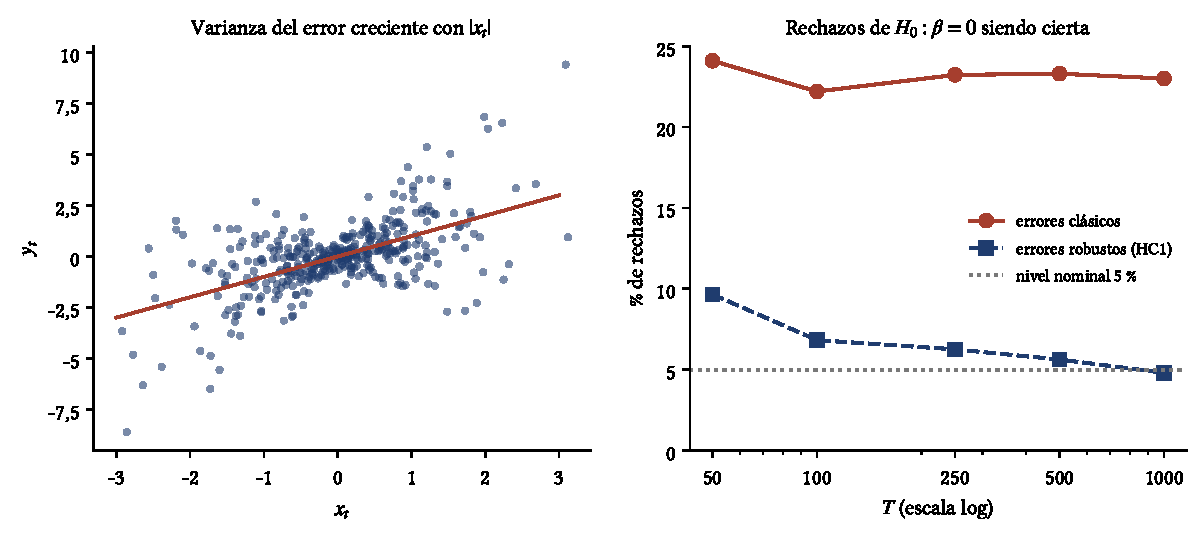
\includegraphics[width=\linewidth]{graficos/cap04_fig_hetero.pdf}
\caption{Izquierda: datos simulados con $\beta=1$ cuya varianza del error crece con $|x_t|$: la nube tiene
forma de embudo, más ancha en los extremos. Derecha: porcentaje de rechazos de una hipótesis cierta con la
prueba $t$ al 5\,\%, en 4\,000 simulaciones por tamaño de muestra. Con errores clásicos se rechaza en torno
al 23\,\% de las veces sin importar $T$; con errores robustos, el porcentaje se acerca al 5\,\%.}
\label{fig:hetero}
\end{figure}

\subsection{Pruebas de heterocedasticidad}

\begin{definicion}[Pruebas de Breusch-Pagan y de White]
Se estima la regresión auxiliar de $\hat\varepsilon_t^2$ sobre una constante y un conjunto de $q$ variables
$\bm z_t$, y se calcula $LM=T\cdot R^2_{\mathrm{aux}}$. Bajo homocedasticidad, $LM$ converge a una
$\chi^2_q$. En la prueba de \emph{Breusch-Pagan} (en la versión de Koenker), $\bm z_t$ son los regresores
originales; en la de \emph{White}, son los regresores, sus cuadrados y sus productos cruzados.
\end{definicion}

\begin{observacion}
La diferencia importa en el modelo de mercado. Si la varianza del residuo crece con $|x_t|$ (tanto en las
subidas como en las caídas del mercado), su relación con $x_t$ es simétrica y no lineal: la regresión
auxiliar sobre $x_t$ no la detecta, pero la regresión sobre $x_t$ y $x_t^2$ sí.
\end{observacion}

% ---------------------------------------------------------------------
\section{Autocorrelación y errores de Newey-West}
% ---------------------------------------------------------------------

\subsection{La varianza de largo plazo}

Escribimos $\sqrt T(\hat{\bm\beta}-\bm\beta)=\bigl(\tfrac1T\bm X'\bm X\bigr)^{-1}\tfrac{1}{\sqrt T}\sum_t\bm u_t$,
con $\bm u_t=\bm x_t\varepsilon_t$. Toda la incertidumbre de $\hat{\bm\beta}$ proviene de la suma
$\sum_t\bm u_t$. Si los $\bm u_t$ están autocorrelacionados, su varianza no es la suma de varianzas: es la
misma situación que la agregación temporal de rendimientos (Proposición~\ref{prop:agregmom}).

\begin{proposicion}[Varianza de largo plazo]\label{prop:vlp}
Si $\bm u_t$ es estacionario con media cero y autocovarianzas $\bm\Gamma_j=\E[\bm u_t\bm u_{t-j}']$, entonces
\[
  \Var\Bigl(\frac1{\sqrt T}\sum_{t=1}^T\bm u_t\Bigr)=\bm\Gamma_0+\sum_{j=1}^{T-1}\Bigl(1-\frac jT\Bigr)
  \bigl(\bm\Gamma_j+\bm\Gamma_j'\bigr)\ \longrightarrow\ \bm S=\bm\Gamma_0+\sum_{j=1}^{\infty}\bigl(\bm\Gamma_j+\bm\Gamma_j'\bigr).
\]
\end{proposicion}

\begin{proof}
La varianza de la suma es la suma de todas las covarianzas. Agrupamos los pares $(t,s)$ por su distancia:
hay $T$ pares con $t=s$; para cada $j\ge1$ hay $T-j$ pares con $t-s=j$, que aportan $\bm\Gamma_j$, y $T-j$
con $s-t=j$, que aportan $\bm\Gamma_j'$:
\begin{align*}
  \Var\Bigl(\frac1{\sqrt T}\sum_{t=1}^T\bm u_t\Bigr)
    &= \frac1T\sum_{t=1}^T\sum_{s=1}^T\E[\bm u_t\bm u_s']\\
    &= \frac1T\Bigl[T\,\bm\Gamma_0+\sum_{j=1}^{T-1}(T-j)\,\bm\Gamma_j+\sum_{j=1}^{T-1}(T-j)\,\bm\Gamma_j'\Bigr]\\
    &= \bm\Gamma_0+\sum_{j=1}^{T-1}\Bigl(1-\frac jT\Bigr)\bigl(\bm\Gamma_j+\bm\Gamma_j'\bigr).
\end{align*}
Si las autocovarianzas son sumables, el último término converge a $\sum_{j\ge1}(\bm\Gamma_j+\bm\Gamma_j')$
cuando $T\to\infty$.
\end{proof}

La matriz $\bm S$ se llama \emph{varianza de largo plazo}. Con errores no autocorrelacionados se reduce a
$\bm\Gamma_0$, que es lo que estima el relleno de White.

\begin{definicion}[Estimador de Newey-West]
Con $\hat{\bm u}_t=\bm x_t\hat\varepsilon_t$ y $\hat{\bm\Gamma}_j=\sum_{t=j+1}^T\hat{\bm u}_t\hat{\bm u}_{t-j}'$,
\[
  \widehat{\bm V}_{\mathrm{NW}}=(\bm X'\bm X)^{-1}\Bigl[\hat{\bm\Gamma}_0+\sum_{j=1}^{L}\Bigl(1-\frac{j}{L+1}\Bigr)
  \bigl(\hat{\bm\Gamma}_j+\hat{\bm\Gamma}_j'\bigr)\Bigr](\bm X'\bm X)^{-1}.
\]
\end{definicion}

Los pesos $1-j/(L+1)$ (núcleo de Bartlett) decrecen linealmente hasta cero. Newey y West (1987) mostraron que
con ellos la matriz estimada es siempre semidefinida positiva (una varianza nunca negativa), lo que no
ocurriría con pesos iguales a 1, y que el estimador es consistente si $L$ crece con $T$, pero más despacio.
Una regla práctica habitual es $L=\lfloor4(T/100)^{2/9}\rfloor$ (Newey y West, 1994), que da $L=6$ con
$T=819$ meses. Con $L=0$ el estimador se reduce a HC0, por lo que Newey-West es robusto a la vez a la
heterocedasticidad y a la autocorrelación (HAC, por sus siglas en inglés).

\subsection{Una prueba de autocorrelación robusta}

Volvemos a la deuda del Capítulo~\ref{cap:hechos}.

\begin{proposicion}[Autocorrelación muestral bajo heterocedasticidad condicional]\label{prop:acfrob}
Si $r_t$ es estacionario, con media cero, cuarto momento finito y $\E[r_t\mid\mathcal F_{t-1}]=0$ (como el
proceso de la Proposición~\ref{prop:mds}), entonces, para cada $j\ge1$,
\[
  \sqrt T\,\hat\rho_j\xrightarrow{d}N\Bigl(0,\ \frac{\E[r_t^2r_{t-j}^2]}{\sigma^4}\Bigr).
\]
\end{proposicion}

\begin{proof}[Esbozo de demostración]
Como la media es cero, en muestras grandes
\begin{align*}
  \sqrt T\,\hat\rho_j &\approx \frac{\frac{1}{\sqrt T}\sum_tr_t\,r_{t-j}}{\frac1T\sum_tr_t^2},\\
  \frac1T\sum_tr_t^2  &\xrightarrow{p}\sigma^2 .
\end{align*}
En el numerador, $v_t=r_t\,r_{t-j}$ es una diferencia de martingala:
\begin{align*}
  \E[v_t\mid\mathcal F_{t-1}] &= \E[r_t\,r_{t-j}\mid\mathcal F_{t-1}]\\
                              &= r_{t-j}\,\E[r_t\mid\mathcal F_{t-1}]\\
                              &= 0 .
\end{align*}
Por tanto no está autocorrelacionada, y el teorema central del límite para diferencias de martingala da
\begin{align*}
  \frac1{\sqrt T}\sum_tv_t &\xrightarrow{d}N\bigl(0,\ \E[v_t^2]\bigr) = N\bigl(0,\ \E[r_t^2r_{t-j}^2]\bigr).
\end{align*}
Por el teorema de Slutsky,
\begin{align*}
  \sqrt T\,\hat\rho_j &\xrightarrow{d} N\Bigl(0,\ \frac{\E[r_t^2r_{t-j}^2]}{\sigma^4}\Bigr). && \qedhere
\end{align*}
\end{proof}

Si los $r_t$ son i.i.d., $\E[r_t^2r_{t-j}^2]=\sigma^4$ y se recupera la banda de Bartlett. Con agrupamiento de
volatilidad, $\E[r_t^2r_{t-j}^2]=\sigma^4+\Cov(r_t^2,r_{t-j}^2)>\sigma^4$ y la varianza verdadera es mayor. La
versión muestral da una banda robusta, $\pm1{,}96\sqrt{\hat v_j}$ con
$\hat v_j=\sum_tr_t^2r_{t-j}^2/(\sum_tr_t^2)^2$, y una prueba conjunta $Q^*(m)=\sum_{j=1}^m\hat\rho_j^2/\hat v_j$,
que se compara con una $\chi^2_m$. Esta es una versión simple, que ignora las covarianzas entre los $\hat\rho_j$
de distintos rezagos; Lobato, Nankervis y Savin (2001) desarrollan versiones más generales.

\subsection{Regresiones con horizontes traslapados}

En finanzas es frecuente preguntar si una variable predice el rendimiento de los próximos $k$ períodos y
usar, para ganar observaciones, rendimientos de $k$ meses que se calculan cada mes. Los datos se
\emph{traslapan}: el rendimiento de enero a diciembre y el de febrero a enero comparten once meses.

\begin{proposicion}[Correlación inducida por el traslape]\label{prop:traslape}
Si los rendimientos de un período $g_t$ son no correlacionados con varianza $\sigma^2$ y
$y_t=\sum_{i=1}^kg_{t+i}$, entonces $\operatorname{Corr}(y_t,y_{t-j})=(k-j)/k$ para $0\le j<k$, y cero para
$j\ge k$.
\end{proposicion}

\begin{proof}
Escribimos ambas sumas:
\begin{align*}
  y_t     &= g_{t+1}+g_{t+2}+\cdots+g_{t+k},\\
  y_{t-j} &= g_{t-j+1}+g_{t-j+2}+\cdots+g_{t-j+k}.
\end{align*}
Para $0\le j<k$ comparten exactamente los $k-j$ rendimientos $g_{t+1},\dots,g_{t-j+k}$. Como los $g$ no
están correlacionados, solo esos términos comunes aportan covarianza:
\begin{align*}
  \Cov(y_t,y_{t-j})            &= \sum_{i=t+1}^{t-j+k}\Var(g_i)\\
                               &= (k-j)\,\sigma^2,\\
  \Var(y_t)                    &= k\,\sigma^2,\\
  \operatorname{Corr}(y_t,y_{t-j}) &= \frac{(k-j)\,\sigma^2}{k\,\sigma^2}\\
                               &= \frac{k-j}{k}.
\end{align*}
Para $j\ge k$ no hay términos comunes y la covarianza es cero.
\end{proof}

\begin{proposicion}[Factor de inflación con un predictor persistente]\label{prop:inflacion}
Suponga que el predictor $x_t$, centrado, es estacionario e independiente del error $\varepsilon_t$, con
autocorrelaciones $\rho_x(j)$ y $\rho_\varepsilon(j)$. Entonces, en muestras grandes, el cociente entre la
varianza verdadera de $\hat\beta$ y la que estima la fórmula clásica es
\[
  1+2\sum_{j=1}^{\infty}\rho_x(j)\,\rho_\varepsilon(j).
\]
\end{proposicion}

\begin{proof}
La incertidumbre de $\hat\beta$ proviene de $\sum_tu_t$ con $u_t=x_t\varepsilon_t$. Por independencia entre
$x$ y $\varepsilon$:
\begin{align*}
  \E[u_t\,u_{t-j}] &= \E[x_t\,x_{t-j}\,\varepsilon_t\,\varepsilon_{t-j}]\\
                   &= \E[x_t\,x_{t-j}]\,\E[\varepsilon_t\,\varepsilon_{t-j}]\\
                   &= \gamma_x(j)\,\gamma_\varepsilon(j)\\
                   &= \gamma_x(0)\,\gamma_\varepsilon(0)\,\rho_x(j)\,\rho_\varepsilon(j).
\end{align*}
Por la Proposición~\ref{prop:vlp}, la varianza de largo plazo es
\begin{align*}
  S &= \E[u_t^2]+2\sum_{j\ge1}\E[u_t\,u_{t-j}]\\
    &= \gamma_x(0)\,\gamma_\varepsilon(0)\Bigl[1+2\sum_{j\ge1}\rho_x(j)\,\rho_\varepsilon(j)\Bigr].
\end{align*}
La fórmula clásica usa solo $\E[u_t^2]=\gamma_x(0)\gamma_\varepsilon(0)$, así que el cociente es
\begin{align*}
  \frac{S}{\gamma_x(0)\,\gamma_\varepsilon(0)} &= 1+2\sum_{j\ge1}\rho_x(j)\,\rho_\varepsilon(j). && \qedhere
\end{align*}
\end{proof}

Con traslape de $k$ períodos, $\rho_\varepsilon(j)=(k-j)/k$, y si el predictor es muy persistente
($\rho_x(j)\approx1$), el factor es aproximadamente $1+2\sum_{j=1}^{k-1}(k-j)/k=k$: la varianza clásica
subestima la verdadera en un factor cercano a $k$, y los errores estándar en un factor cercano a $\sqrt k$.
Con $k=12$, los estadísticos $t$ clásicos están inflados unas $3{,}5$ veces. La Figura~\ref{fig:traslape}
lo muestra: con un predictor persistente pero \emph{completamente inútil}, la prueba clásica ``encuentra''
predictibilidad el 56\,\% de las veces. Newey-West corrige buena parte del problema, pero en muestras
finitas sigue rechazando de más (15,8\,\%); usar solo observaciones sin traslape da un tamaño correcto
(6,4\,\%), a costa de perder datos.

\begin{figure}[ht]
\centering
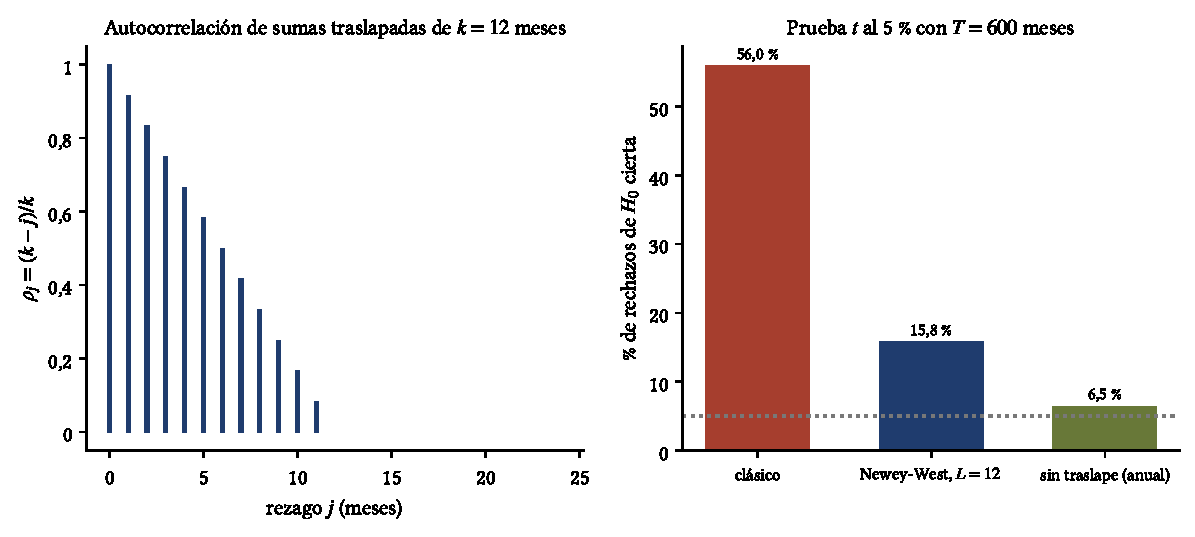
\includegraphics[width=\linewidth]{graficos/cap04_fig_traslape.pdf}
\caption{Izquierda: autocorrelación teórica de rendimientos de 12 meses calculados cada mes; decrece en línea
recta hasta anularse en el rezago 12 (Proposición~\ref{prop:traslape}). Derecha: porcentaje de rechazos de
$H_0:\beta=0$, que es cierta, al regresar rendimientos traslapados sobre un predictor independiente y muy
persistente ($\phi=0{,}98$), en 2\,000 simulaciones con $T=600$.}
\label{fig:traslape}
\end{figure}

\begin{observacion}
Las regresiones predictivas con predictores muy persistentes tienen además otro problema, el \emph{sesgo
de Stambaugh} (1999): si las innovaciones del predictor están correlacionadas con las del rendimiento, como
ocurre con la razón dividendo/precio, $\hat\beta$ está sesgado en muestras finitas. Lo retomaremos en el
Capítulo~6.
\end{observacion}

% ---------------------------------------------------------------------
\section{Cambios estructurales}
% ---------------------------------------------------------------------

En setenta años pueden cambiar la regulación, la tecnología y la composición de las empresas de un sector.
Si la beta cambió y estimamos una sola recta, obtenemos un promedio de dos regímenes que no describe ninguno
de ellos (Figura~\ref{fig:quiebre}).

\begin{figure}[ht]
\centering
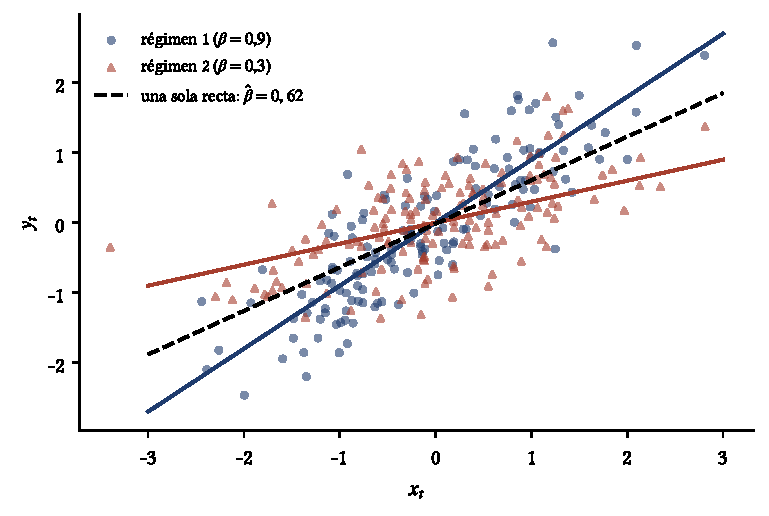
\includegraphics[width=0.66\linewidth]{graficos/cap04_fig_quiebre.pdf}
\caption{Datos simulados con un cambio de régimen: la pendiente es 0,9 en el primero (círculos) y 0,3 en el
segundo (triángulos). Una sola recta (línea discontinua) da una pendiente intermedia de 0,62, que no
representa ninguno de los dos regímenes.}
\label{fig:quiebre}
\end{figure}

\begin{definicion}[Prueba de Chow]
Para una fecha de quiebre conocida $\tau$, se estima el modelo con toda la muestra (suma de residuos al
cuadrado $\mathrm{SRC}$) y por separado antes y después de $\tau$ ($\mathrm{SRC}_1$ y $\mathrm{SRC}_2$). Con $k$
parámetros por régimen,
\[
  F=\frac{(\mathrm{SRC}-\mathrm{SRC}_1-\mathrm{SRC}_2)/k}{(\mathrm{SRC}_1+\mathrm{SRC}_2)/(T-2k)} .
\]
Con errores normales, homocedásticos y no correlacionados, $F$ sigue una distribución $F_{k,\,T-2k}$ bajo la
hipótesis nula de que los parámetros no cambiaron.
\end{definicion}

La prueba de Chow equivale a estimar un solo modelo con una variable indicadora $D_t=\mathbb 1\{t\ge\tau\}$
y sus interacciones con los regresores, y a probar que los coeficientes de esos términos son cero. Esta
forma permite usar errores robustos: se calcula la prueba de Wald con la matriz HC1 o Newey-West, y se compara
con una $\chi^2_k$.

\paragraph{Fecha desconocida.} Si la fecha se elige mirando los datos, por ejemplo donde $F$ es máximo, los
valores críticos de la $F$ ya no sirven: el máximo de muchas $F$ es mucho mayor que una $F$ típica. Andrews
(1993) obtuvo la distribución asintótica de $\sup F$ sobre las fechas entre el 15\,\% y el 85\,\% de la
muestra. Para $k=2$, el valor crítico al 5\,\% del estadístico de Wald ($=k\cdot\sup F$) es de
aproximadamente 11,8; nuestra simulación con puentes brownianos da 11,70, es decir, $\sup F$ crítico
$\approx5{,}85$ (Ejercicio propuesto~4.6).

\paragraph{CUSUM.} Brown, Durbin y Evans (1975) propusieron vigilar la estabilidad con los \emph{residuos
recursivos}: el error de pronóstico de $y_t$ con el modelo estimado hasta $t-1$, estandarizado,
\[
  w_t=\frac{y_t-\bm x_t'\hat{\bm\beta}_{t-1}}{\sqrt{1+\bm x_t'(\bm X_{t-1}'\bm X_{t-1})^{-1}\bm x_t}} .
\]
Con errores normales e i.i.d. y parámetros estables, los $w_t$ son i.i.d. $N(0,\sigma^2)$. Su suma acumulada
estandarizada, $W_t=\sum_{s\le t}w_s/\hat\sigma_w$, se mueve como un paseo aleatorio alrededor de cero; un
cambio en los parámetros produce errores de pronóstico sistemáticos y $W_t$ se desvía. Las bandas al 5\,\%
son $\pm0{,}948\bigl[\sqrt{T-k}+2(t-k)/\sqrt{T-k}\bigr]$.

% ---------------------------------------------------------------------
\section{Ejercicios resueltos}
% ---------------------------------------------------------------------

\begin{ejresuelto}{Heterocedasticidad en la beta de los servicios públicos}\label{ej:white}
\enunciado Con el modelo de mercado de \texttt{Utils} (Ejercicio~\ref{ej:utils}): (a) aplique las pruebas de
Breusch-Pagan y de White; (b) calcule los errores estándar clásicos, HC0 y HC1 con la matriz sándwich;
(c) repita las pruebas de $\alpha=0$ y $\beta=1$.

\solucion
\paso{Paso 1. Pruebas.} Breusch-Pagan: $LM=6{,}19$ con 1 grado de libertad, $p=0{,}013$. White:
$LM=36{,}56$ con 2 grados de libertad, $p\approx10^{-8}$. Las dos rechazan la homocedasticidad, pero la de
White con mucha más fuerza: la Figura~\ref{fig:white} muestra que los residuos al cuadrado crecen tanto
con las subidas como con las caídas del mercado, una relación en forma de U que solo el término $x_t^2$ capta.

\paso{Paso 2. Errores estándar.} Para $\hat\beta$: clásico $0{,}02497$, HC0 $0{,}03312$ y HC1 $0{,}03316$.
El cociente entre el robusto y el clásico es
\begin{align*}
  \frac{\operatorname{ee}_{\mathrm{HC1}}(\hat\beta)}{\operatorname{ee}_{\text{clásico}}(\hat\beta)}
    &= \frac{0{,}03316}{0{,}02497}\\
    &= 1{,}328 :
\end{align*}
el error estándar robusto es un 33\,\% mayor. Para $\hat\alpha$ el cambio es mínimo ($0{,}00107$ a
$0{,}00110$), porque la constante no interactúa con la forma de la heterocedasticidad.

\paso{Paso 3. Pruebas revisadas.} Con los errores HC1:
\begin{align*}
  t_{\mathrm{HC1}}(\beta=1)  &= \frac{0{,}54087-1}{0{,}03316}\\
                             &= -13{,}85,\\
  t_{\mathrm{HC1}}(\alpha=0) &= \frac{0{,}0024625}{0{,}0011043}\\
                             &= 2{,}23 .
\end{align*}
La beta sigue siendo claramente menor que 1 (antes, $t=-18{,}39$) y la alfa sigue siendo significativa al
5\,\% (antes, $t=2{,}30$).

\codigoweb{cap04_ej01}
\salidaR{cap04_ej01_R.txt}
\lectura{cap04_ej01}

\RvsPy Programamos la matriz sándwich en ambos lenguajes para que el cálculo sea transparente. La
expresión \texttt{X * e} multiplica cada fila de $\bm X$ por su residuo: en R funciona porque el vector
\texttt{e} se recicla por columnas; en NumPy hay que convertirlo en columna con \texttt{e[:, None]}. En la
práctica, R ofrece estas matrices en el paquete \texttt{sandwich} y Python en la opción \texttt{cov\_type}
de \texttt{statsmodels}, que usamos como comprobación.

\begin{figure}[ht]
\centering
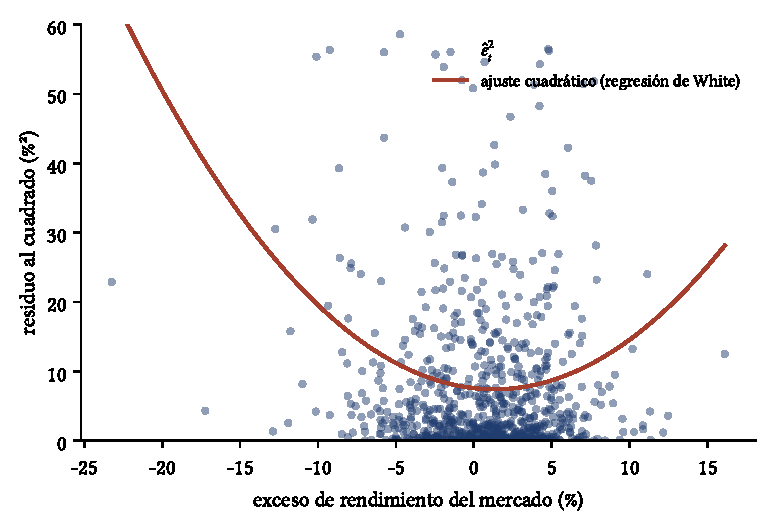
\includegraphics[width=0.68\linewidth]{graficos/cap04_fig_white.pdf}
\caption{Residuos al cuadrado del modelo de mercado de \texttt{Utils} frente al exceso de rendimiento del
mercado. La parábola ajustada (la regresión auxiliar de White) muestra que la varianza del residuo crece en
ambos extremos.}
\label{fig:white}
\end{figure}

\begin{conclusion}
Hay heterocedasticidad clara, y los errores estándar clásicos de la beta la subestiman en un tercio. Las
conclusiones del Capítulo~\ref{cap:capm} sobre \texttt{Utils} se mantienen, pero con menos holgura de la que
parecía.
\end{conclusion}
\end{ejresuelto}

\begin{ejresuelto}{¿Sobreviven las alfas del CAPM a los errores robustos?}\label{ej:alfasrob}
\enunciado Repita el Ejercicio~\ref{ej:industrias} con errores HC1 y Newey-West ($L=6$). ¿Cuántas alfas
siguen siendo significativas? ¿Cuánto crecen los errores estándar de las betas?

\solucion
\paso{Paso 1. Rezagos.} Con $T=819$, la regla de Newey y West da
\begin{align*}
  L &= \Bigl\lfloor 4\Bigl(\frac{T}{100}\Bigr)^{2/9}\Bigr\rfloor\\
    &= \bigl\lfloor 4\,(8{,}19)^{2/9}\bigr\rfloor\\
    &= \lfloor 4\times1{,}5957\rfloor\\
    &= \lfloor 6{,}38\rfloor\\
    &= 6 .
\end{align*}

\paso{Paso 2. Alfas.} Las cuatro alfas significativas con errores clásicos siguen siéndolo con HC1 y con
Newey-West: \texttt{NoDur} (de $t=2{,}87$ a $2{,}27$ con Newey-West), \texttt{Hlth} (de $2{,}49$ a
$2{,}32$), \texttt{Utils} (de $2{,}30$ a $2{,}25$) y \texttt{Other} (de $-2{,}24$ a $-2{,}16$). La evidencia
contra el CAPM del Capítulo~\ref{cap:capm} no era un artefacto de los errores estándar.

\paso{Paso 3. Betas.} Los errores estándar de las betas crecen mucho más: en promedio, el de Newey-West es
1,6 veces el clásico, y en \texttt{NoDur} es el doble. Newey-West supera a HC1 en las doce industrias,
lo que indica que los productos $x_t\hat\varepsilon_t$ están autocorrelacionados: es la huella del
agrupamiento de volatilidad. Con estos errores, \texttt{Money} ($t(\beta=1)=1{,}61$) se suma a
\texttt{Shops} como industria cuya beta no se distingue de 1.

\codigoweb{cap04_ej02}
\salidaR{cap04_ej02_R.txt}
\lectura{cap04_ej02}

\RvsPy Para que Python reproduzca la fórmula de Newey-West sin correcciones adicionales hay que indicar
\texttt{use\_correction=False} en \texttt{statsmodels}; por defecto multiplica la matriz por $T/(T-k)$. Es
un buen ejemplo de por qué conviene saber qué calcula cada función: las dos versiones son válidas, pero
difieren en la tercera cifra decimal.

\begin{figure}[ht]
\centering
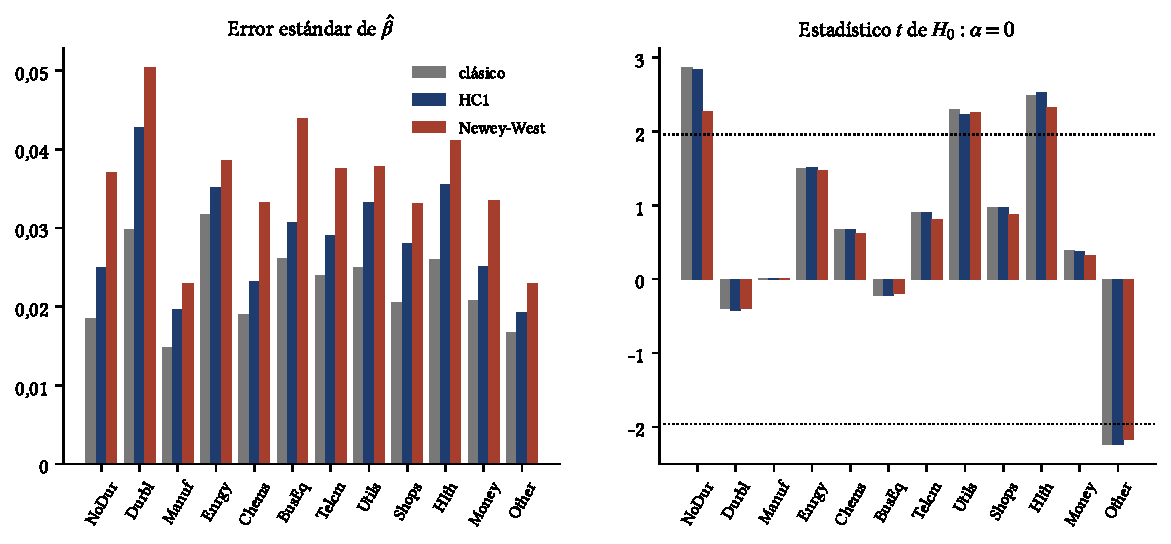
\includegraphics[width=\linewidth]{graficos/cap04_fig_robustos.pdf}
\caption{Izquierda: error estándar de $\hat\beta$ con los tres métodos; el de Newey-West es el mayor en todas
las industrias. Derecha: estadístico $t$ de $\alpha=0$; las barras que superan las líneas punteadas
($\pm1{,}96$) son las mismas con los tres métodos.}
\label{fig:robustos}
\end{figure}

\begin{conclusion}
Los errores robustos no cambian las conclusiones sobre las alfas, pero sí la precisión con que conocemos las
betas, que es un 60\,\% menor de lo que indicaban los errores clásicos. En aplicaciones financieras, los
errores HAC deberían ser la opción por defecto.
\end{conclusion}
\end{ejresuelto}

\begin{ejresuelto}{La deuda del Capítulo 2: autocorrelación del Brent con bandas robustas}\label{ej:acfrob}
\enunciado Con los rendimientos diarios del Brent, calcule las diez primeras autocorrelaciones con las bandas
de Bartlett y con las bandas robustas de la Proposición~\ref{prop:acfrob}. Compare la prueba de Ljung-Box con
la versión robusta $Q^*(10)$.

\solucion
\paso{Paso 1. Bandas.} La banda de Bartlett es $\pm0{,}0205$ en todos los rezagos. Las robustas van de
$\pm0{,}038$ (rezago 8) a $\pm0{,}090$ (rezago 1): entre 1,9 y 4,4 veces más anchas.

\paso{Paso 2. Rezagos ``significativos''.} Con la banda clásica, los rezagos 2, 8 y 10 parecían
significativos ($t=-2{,}47$; $1{,}98$; $-2{,}69$). Con la robusta, sus estadísticos son $-1{,}12$; $1{,}07$ y
$-0{,}87$: ninguno se acerca a la significancia.

\paso{Paso 3. Prueba conjunta.} Ljung-Box da $Q(10)=25{,}74$, $p=0{,}0041$; la versión robusta da
$Q^*(10)=4{,}67$, $p=0{,}912$.

\codigoweb{cap04_ej03}
\salidaR{cap04_ej03_R.txt}
\lectura{cap04_ej03}

\RvsPy Los dos programas siguen exactamente las fórmulas de la Proposición~\ref{prop:acfrob} sobre los
rendimientos centrados. En R convertimos el resultado de \texttt{sapply} en un \texttt{data.frame} para
acceder a las columnas por nombre (\texttt{res\$rho}).

\begin{figure}[ht]
\centering
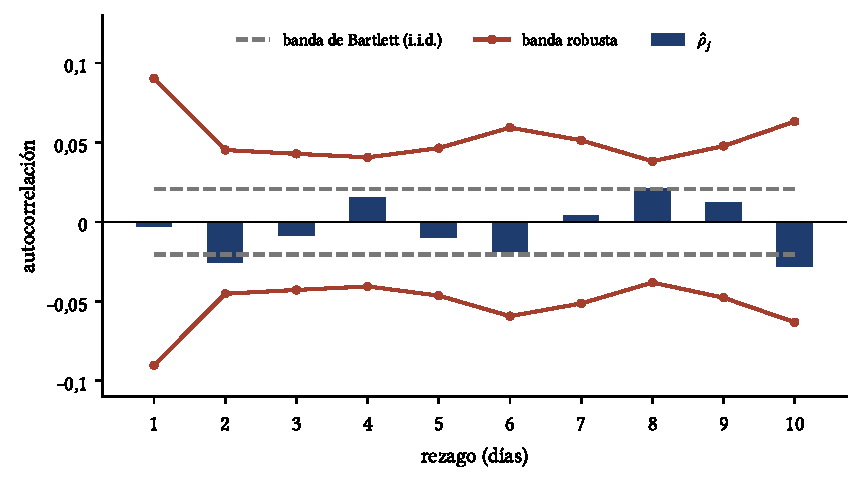
\includegraphics[width=0.78\linewidth]{graficos/cap04_fig_acfrobusta.pdf}
\caption{Autocorrelaciones del Brent con la banda de Bartlett (gris), válida solo con datos i.i.d., y con la
banda robusta (roja). Ninguna autocorrelación sale de la banda robusta.}
\label{fig:acfrobusta}
\end{figure}

\begin{conclusion}
El rechazo de Ljung-Box en el Capítulo~\ref{cap:hechos} era un artefacto del agrupamiento de volatilidad. Con
inferencia válida, no hay evidencia de autocorrelación en los rendimientos diarios del Brent, en línea con la
eficiencia débil del mercado petrolero, que estudiaremos en el Capítulo~7.
\end{conclusion}
\end{ejresuelto}

\begin{ejresuelto}{¿Predice la razón dividendo/precio el rendimiento bursátil?}\label{ej:dprediccion}
\enunciado Con el S\&P 500 de Shiller (1871--2023), regrese el rendimiento total logarítmico de los próximos
12 meses sobre $\ln(D_t/P_t)$, usando todos los meses (datos traslapados). Compare los errores estándar
clásicos, de Newey-West con $L=12$ y $L=24$, y la regresión con un solo dato por año (eneros, sin traslape).

\solucion
\paso{Paso 1. Estimación.} Con 1\,818 meses (enero de 1871 a junio de 2022 como fechas iniciales),
$\hat b=0{,}0412$ y $R^2=0{,}0107$. El signo es el que predice la teoría (Campbell y Shiller, 1988): cuando los
precios están altos en relación con los dividendos, los rendimientos futuros tienden a ser menores.

\paso{Paso 2. Inferencia.} Con errores clásicos, $t=4{,}43$: predictibilidad ``muy significativa''. Con
Newey-West, $t=1{,}46$ ($L=12$) y $t=1{,}35$ ($L=24$). Sin traslape, con 152 eneros, $\hat b=0{,}0334$ y
$t=1{,}09$. Ninguna versión válida es significativa al 5\,\%.

\paso{Paso 3. Comparación con la teoría.} La razón dividendo/precio es extremadamente persistente: su
autocorrelación es $0{,}996$ al primer rezago y $0{,}906$ a los doce meses. Con $\rho_x(j)=0{,}996^{\,j}$ y
$\rho_\varepsilon(j)=(12-j)/12$, la Proposición~\ref{prop:inflacion} da
\begin{align*}
  1+2\sum_{j=1}^{11}0{,}996^{\,j}\,\frac{12-j}{12} &= 1+2\times5{,}406\\
                                                    &= 11{,}81,\\
  \sqrt{11{,}81}                                    &= 3{,}44 .
\end{align*}
Los errores estándar verdaderos deberían ser unas 3,44 veces los clásicos. En los datos,
\begin{align*}
  \frac{\operatorname{ee}_{\mathrm{NW}}(\hat b)}{\operatorname{ee}_{\text{clásico}}(\hat b)} &= \frac{0{,}0283}{0{,}0093}\\
                                                                                         &= 3{,}04 :
\end{align*}
la teoría explica casi todo el desajuste.

\codigoweb{cap04_ej04}
\salidaR{cap04_ej04_R.txt}
\lectura{cap04_ej04}

\RvsPy La serie de Shiller incluye los dividendos anuales acumulados de cada mes; el rendimiento mensual
total suma la doceava parte al precio. En los dos lenguajes cortamos la muestra en junio de 2023, último mes
con dividendo publicado; si no se hace, los dividendos iguales a cero producen $\ln 0=-\infty$ y la regresión
falla o, peor, descarta observaciones sin avisar.

\begin{figure}[ht]
\centering
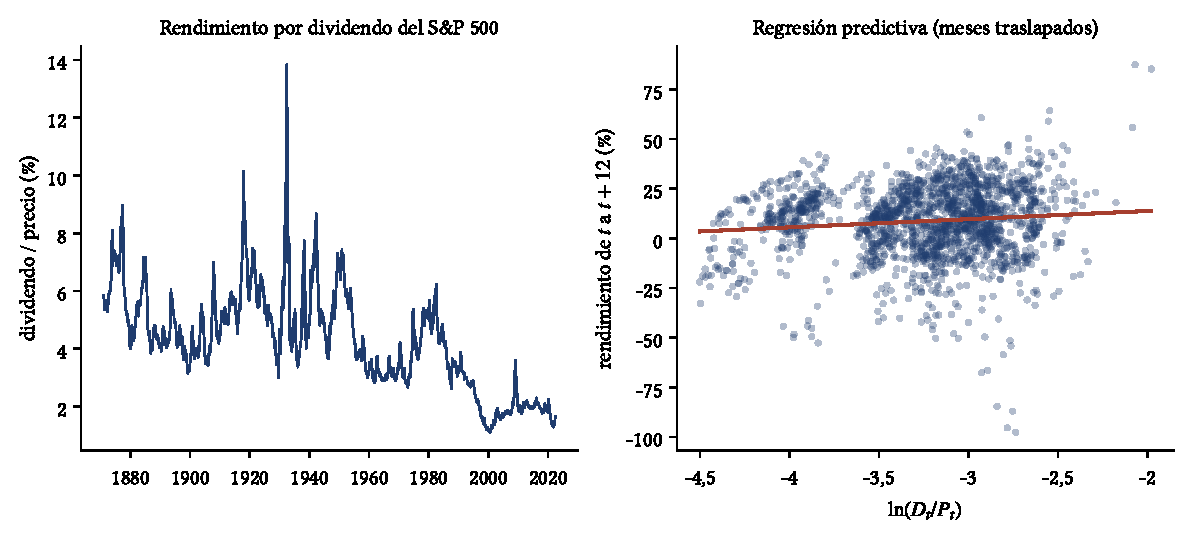
\includegraphics[width=\linewidth]{graficos/cap04_fig_dividendos.pdf}
\caption{Izquierda: rendimiento por dividendo del S\&P 500, una serie muy persistente que tocó su
mínimo histórico (1,1\,\% en agosto de 2000). Derecha: rendimiento de los 12 meses siguientes frente al logaritmo de la razón
dividendo/precio. La pendiente positiva es pequeña frente a la dispersión, y los puntos vecinos no son
observaciones independientes.}
\label{fig:dividendos}
\end{figure}

\begin{conclusion}
La aparente predictibilidad del mercado accionario con la razón dividendo/precio desaparece cuando se corrige
la inferencia por el traslape. Sumado al sesgo de Stambaugh, este ejemplo muestra por qué la literatura sobre
predictibilidad de rendimientos exige errores HAC, pruebas sin traslape y evaluación fuera de muestra.
\end{conclusion}
\end{ejresuelto}

\begin{ejresuelto}{¿Cambió la beta de los servicios públicos tras la desregulación eléctrica?}\label{ej:chow}
\enunciado En octubre de 1992 se promulgó en EE.\,UU. la Ley de Política Energética, que abrió a la
competencia la generación eléctrica mayorista. Con el modelo de mercado de \texttt{Utils}: (a) aplique la
prueba de Chow con quiebre en octubre de 1992 y su versión robusta; (b) calcule $\sup F$ sin fijar la fecha;
(c) aplique la prueba CUSUM.

\solucion
\paso{Paso 1. Chow.} $F=11{,}43$ frente a un valor crítico de $F_{2,815}$ al 5\,\% de $3{,}01$ ($p=1{,}3\times10^{-5}$).
La beta pasa de $0{,}629$ antes de la ley a $0{,}384$ después, y la alfa anual, de $2{,}19$\,\% a $4{,}35$\,\%.
Como hay heterocedasticidad (Ejercicio~\ref{ej:white}), repetimos con la prueba de Wald robusta: $W=10{,}97$
frente a $\chi^2_2=5{,}99$, $p=0{,}004$. El cambio se confirma.

\paso{Paso 2. Fecha desconocida.} El máximo de las $F$ entre el 15\,\% y el 85\,\% de la muestra es
$16{,}69$, en febrero de 1987, muy por encima del valor crítico de Andrews ($\approx5{,}85$). La
Figura~\ref{fig:quiebres} muestra que la $F$ supera el valor crítico en casi todas las fechas entre abril de
1974 y noviembre de 1999: la beta cambió en algún momento de ese período, pero los datos no permiten
fecharlo con precisión, y octubre de 1992 no es la fecha más probable. Sospechar una ley concreta no basta
para atribuirle el cambio.

\paso{Paso 3. CUSUM.} El estadístico nunca cruza sus bandas: su máximo llega al 73\,\% de la banda. La prueba
no detecta el cambio que Chow y $\sup F$ detectan con claridad. No es una contradicción: CUSUM acumula errores
de pronóstico, que se vuelven sistemáticos cuando cambia el nivel de la serie; un cambio en la pendiente con
un regresor de media cercana a cero (el exceso del mercado) produce errores que se compensan entre meses
buenos y malos, y la suma apenas se mueve (Ploberger y Krämer, 1990).

\codigoweb{cap04_ej05}
\salidaR{cap04_ej05_R.txt}
\lectura{cap04_ej05}

\RvsPy Dos trampas de índices. Primero, la fecha de quiebre: en R, \texttt{tb} es la posición (desde 1) del
primer mes del segundo régimen; en Python, la misma fecha es \texttt{tb} desde 0, y los cortes
\texttt{slice(0, tb)} y \texttt{slice(tb, T)} la dejan en el segundo régimen. Segundo, \texttt{np.argmax}
aplicado a un vector sin ningún \texttt{True} devuelve 0, no un aviso: la primera versión de nuestro código
reportaba un cruce falso en marzo de 1949 hasta que lo corregimos.

\begin{figure}[ht]
\centering
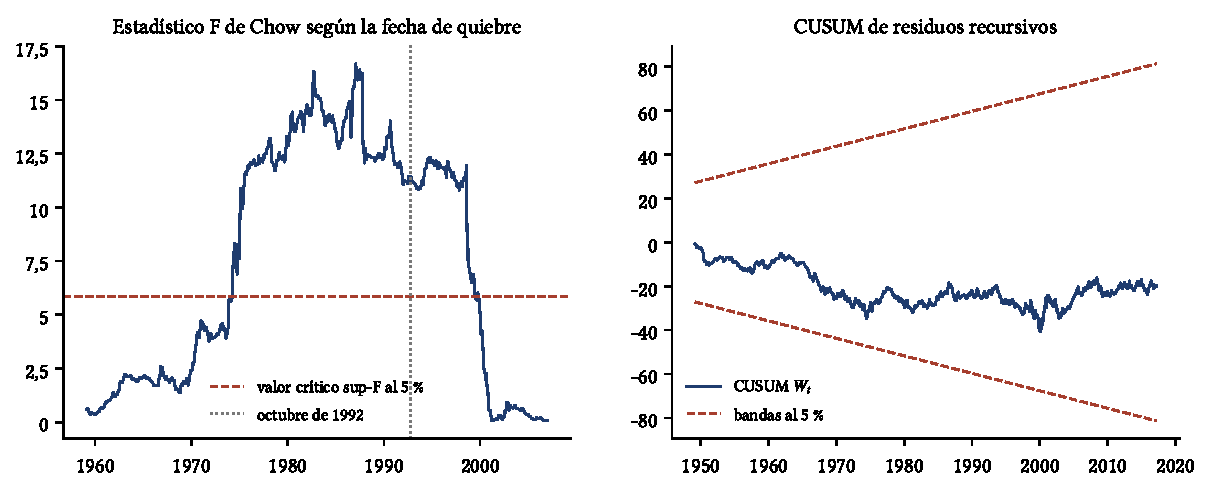
\includegraphics[width=\linewidth]{graficos/cap04_fig_quiebres.pdf}
\caption{Izquierda: estadístico $F$ de Chow para cada fecha posible, con el valor crítico de $\sup F$ al 5\,\%
(línea discontinua) y octubre de 1992 (línea punteada). Derecha: CUSUM de residuos recursivos con sus bandas
al 5\,\%; el estadístico se aleja de cero, pero no las cruza.}
\label{fig:quiebres}
\end{figure}

\begin{conclusion}
La beta de los servicios públicos cayó de forma significativa entre la primera y la segunda mitad de la
muestra, de 0,63 a 0,38, pero la fecha exacta no está bien identificada. Cada prueba responde una pregunta
distinta: Chow evalúa una fecha elegida de antemano, $\sup F$ busca la fecha en los datos con valores
críticos adecuados y CUSUM vigila sobre todo cambios de nivel.
\end{conclusion}
\end{ejresuelto}

% ---------------------------------------------------------------------
\section{Ejercicios propuestos}
% ---------------------------------------------------------------------

\begin{enumerate}[label=\textbf{\thechapter.\arabic*},leftmargin=*,itemsep=6pt]
  \item Demuestre que si $\sigma_t^2$ no está correlacionada con $(x_t-\bar x)^2$, el cociente de la
  Proposición~\ref{prop:mcohetero} es 1, aunque haya heterocedasticidad. ¿Por qué entonces los errores
  robustos de $\hat\alpha$ casi no cambian en el Ejercicio~\ref{ej:white}?

  \item Demuestre que el estimador de Newey-West con $L=1$ es semidefinido positivo en el caso escalar.
  \textit{Pista: escríbalo como $\frac12\sum_t(\hat u_t+\hat u_{t-1})^2$ más términos no negativos.}

  \item Use la Proposición~\ref{prop:inflacion} para calcular el factor de inflación con $k=12$ y
  $\rho_x(j)=\phi^j$ para $\phi=0{,}5;\ 0{,}9;\ 0{,}99$. \textit{Respuesta: 2,67; 8,24 y 11,54.}

  \item Demuestre que la prueba de Chow equivale a la prueba $F$ de que los coeficientes de $D_t$ y
  $D_t\,x_t$ son cero en la regresión con interacciones.

  \item \emph{(Simulación.)} Modifique el código de \texttt{cap04\_figuras\_teoria.py} para que los errores
  sigan un ARCH(1) con $a=0{,}5$ y el regresor sea i.i.d. normal. ¿Cuánto rechaza la prueba $t$ clásica de
  $\beta=0$? ¿Y la prueba con errores HC1?

  \item \emph{(Simulación.)} Simule el valor crítico de $\sup F$ de Andrews: genere dos movimientos
  brownianos independientes en una malla de 2\,000 puntos, construya los puentes $B(\pi)=W(\pi)-\pi W(1)$ y
  calcule $\sup_{\pi\in[0{,}15;\,0{,}85]}\|B(\pi)\|^2/[\pi(1-\pi)]$. Con 20\,000 repeticiones, el cuantil del
  95\,\% debe estar cerca de 11,7 a 11,8.

  \item \emph{(Con datos.)} Repita el Ejercicio~\ref{ej:dprediccion} con dos submuestras, 1871--1945 y
  1946--2022. ¿Es significativa la pendiente en alguna de ellas con Newey-West? ¿Por qué no basta un
  estadístico $t$ alto en la segunda submuestra para concluir que hay predictibilidad?

  \item \emph{(Con datos del BCRP.)} Estime la beta de una acción peruana respecto del índice de la BVL con
  errores clásicos, HC1 y Newey-West, y aplique la prueba de Chow con quiebre en marzo de 2020 (inicio de la
  emergencia sanitaria). ¿Cambió la beta?
\end{enumerate}

% ---------------------------------------------------------------------
\section{Resumen de fórmulas}
% ---------------------------------------------------------------------

\begin{table}[H]
\centering\small
\begin{tabular}{@{}ll@{}}
\toprule
Concepto & Fórmula \\
\midrule
Varianza de MCO (sándwich) & $(\bm X'\bm X)^{-1}\bigl(\sum_t\sigma_t^2\bm x_t\bm x_t'\bigr)(\bm X'\bm X)^{-1}$ \\
White (HC0, HC1) & $\sigma_t^2\to\hat\varepsilon_t^2$;\quad HC1 $=\frac{T}{T-k}$HC0 \\
Breusch-Pagan, White & $LM=T\,R^2_{\mathrm{aux}}\xrightarrow{d}\chi^2_q$ \\
Varianza de largo plazo & $\bm S=\bm\Gamma_0+\sum_{j\ge1}(\bm\Gamma_j+\bm\Gamma_j')$ \\
Newey-West & pesos $1-j/(L+1)$;\quad $L=\lfloor4(T/100)^{2/9}\rfloor$ \\
Autocorrelación robusta & $\hat v_j=\sum_tr_t^2r_{t-j}^2/(\sum_tr_t^2)^2$;\quad $Q^*(m)=\sum_j\hat\rho_j^2/\hat v_j$ \\
Traslape de $k$ períodos & $\rho(j)=(k-j)/k$;\quad inflación $\approx1+2\sum_j\rho_x(j)\rho_\varepsilon(j)$ \\
Chow & $F=\frac{(\mathrm{SRC}-\mathrm{SRC}_1-\mathrm{SRC}_2)/k}{(\mathrm{SRC}_1+\mathrm{SRC}_2)/(T-2k)}$ \\
CUSUM & bandas $\pm0{,}948\bigl[\sqrt{T-k}+2(t-k)/\sqrt{T-k}\bigr]$ \\
\bottomrule
\end{tabular}
\caption{Fórmulas principales del Capítulo 4.}
\end{table}

\section*{Referencias}
\begin{itemize}[leftmargin=*]
  \item Andrews, D. W. K. (1993). Tests for parameter instability and structural change with unknown change
        point. \emph{Econometrica}, 61(4), 821--856.
  \item Breusch, T. S. y Pagan, A. R. (1979). A simple test for heteroscedasticity and random coefficient
        variation. \emph{Econometrica}, 47(5), 1287--1294.
  \item Brown, R. L., Durbin, J. y Evans, J. M. (1975). Techniques for testing the constancy of regression
        relationships over time. \emph{Journal of the Royal Statistical Society, Series B}, 37(2), 149--192.
  \item Campbell, J. Y. y Shiller, R. J. (1988). The dividend-price ratio and expectations of future
        dividends and discount factors. \emph{The Review of Financial Studies}, 1(3), 195--228.
  \item Chow, G. C. (1960). Tests of equality between sets of coefficients in two linear regressions.
        \emph{Econometrica}, 28(3), 591--605.
  \item Koenker, R. (1981). A note on studentizing a test for heteroscedasticity. \emph{Journal of
        Econometrics}, 17(1), 107--112.
  \item Lobato, I., Nankervis, J. C. y Savin, N. E. (2001). Testing for autocorrelation using a modified
        Box-Pierce Q test. \emph{International Economic Review}, 42(1), 187--205.
  \item Newey, W. K. y West, K. D. (1987). A simple, positive semi-definite, heteroskedasticity and
        autocorrelation consistent covariance matrix. \emph{Econometrica}, 55(3), 703--708.
  \item Newey, W. K. y West, K. D. (1994). Automatic lag selection in covariance matrix estimation.
        \emph{The Review of Economic Studies}, 61(4), 631--653.
  \item Ploberger, W. y Krämer, W. (1990). The local power of the CUSUM and CUSUM of squares tests.
        \emph{Econometric Theory}, 6(3), 335--347.
  \item Stambaugh, R. F. (1999). Predictive regressions. \emph{Journal of Financial Economics}, 54(3),
        375--421.
  \item White, H. (1980). A heteroskedasticity-consistent covariance matrix estimator and a direct test for
        heteroskedasticity. \emph{Econometrica}, 48(4), 817--838.
\end{itemize}
